\documentclass[]{article}
\usepackage[utf8]{inputenc}
\usepackage[left=0.5in, right = 0.5in, top = .75in, bottom = .75in]{geometry}
\usepackage[usenames,dvipsnames]{xcolor}
\usepackage{amsmath, amsfonts}
\usepackage{tikz}
\usepackage{comment}
\usepackage[english]{babel}
\usepackage{amsthm}
\usepackage{enumitem}
\usepackage{graphicx}
\usepackage{mathtools}
\usepackage{xstring}
\usepackage{fancyhdr}
\usepackage{subcaption}
\usepackage{float}
\usepackage[most,many,breakable]{tcolorbox}

\newtheorem{theorem}{Theorem}
\newtheorem{corollary}{Corollary}[theorem]
\newtheorem{definition}{Definition}
\newtheorem{lemma}{Lemma}
\renewcommand{\theenumi}{\Alph{enumi}}

\newcommand{\bd}{\textbf}
\newcommand{\del}{\nabla}
\newcommand{\mbf}{\mathbf}
\newcommand{\sbf}{\boldsymbol}
\newcommand{\by}{\times}
\newcommand{\R}{\mathbb R}
\newcommand{\Rn}{{\mathbb R^n}}
\newcommand{\C}{\mathbb C}
\newcommand{\N}{\mathbb N}
\newcommand{\Q}{\mathbb Q}
\newcommand{\cM}{\mathcal M}
\newcommand{\cN}{\mathcal N}
\newcommand{\cX}{\mathcal X}
\newcommand{\cY}{\mathcal Y}
\newcommand{\pcurl}{\nabla \times}
\newcommand{\pdiv}{\nabla \cdot}
\newcommand{\curl}{\mathrm{curl}\,}
\newcommand{\trace}{\mathrm{tr}\,}
\renewcommand{\div}{\mathrm{div}\,}
\renewcommand{\Im}{\mathrm{Im}\,}
\renewcommand{\Re}{\mathrm{Re}\,}
\newcommand{\res}{\mathrm{Res}\,}
\newcommand{\supp}{\mathrm{supp}\,}
\renewcommand{\epsilon}{\varepsilon}
\renewcommand{\bar}{\overline}
\renewcommand{\hat}{\widehat}
\newcommand{\pder}[3][]{%
	\IfEqCase{#2}{%
		{1}{\frac{\partial#1}{\partial #3}}%
	}[\frac{\partial^{#2}}{\partial #3^{#2}}]%
}
\NewDocumentCommand{\paren}{m}{%
	\left(%
	{#1}%
	\right)%
}
\NewDocumentCommand{\bracket}{m}{%
	\left[%
	{#1}%
	\right]%
}

\title{Biharmonic Scattering}
\author{Kale Stahl}

%\pagestyle{fancy}
%\fancyhf{}
%\makeatletter
%\lhead{\@title}
%\chead{\@date}
%\rhead{\@author}
%\makeatother

\definecolor{boiler-gold}{RGB}{207, 185, 145}
\definecolor{boiler-dust}{RGB}{235, 217, 159}
\definecolor{boiler-steam}{RGB}{196, 191, 192}
\definecolor{background}{RGB}{230, 230, 250}
\definecolor{frame}{RGB}{153, 50, 204}
\definecolor{hint}{RGB}{216, 191, 216}

\newtcbtheorem[auto counter]{problem}{Problem\refstepcounter{problem}}{%
	enhanced,
	colback=background,
	colframe=frame,
	fonttitle=\bfseries,
	description color=boiler-steam
}{pr}

\newtcbtheorem{tcbtheorem}{Theorem}{%
	enhanced,
	colback=background,
	colframe=frame,
	fonttitle=\bfseries,
	description color=boiler-steam
}{pr}

\newenvironment{solution}{%
	\begin{tcolorbox}[breakable,colback=white,colframe=frame, enhanced]
		\bd{Solution to Problem~\theproblem:}}{%
		\hfill $\square$
	\end{tcolorbox}
	\vspace{.5cm}}
\newenvironment{hint}{%
	\begin{tcolorbox}[breakable,colback=hint,colframe=frame]
		\bd{Hint:}\itshape}
	{%
\end{tcolorbox}}

\begin{document}
	
	\maketitle
	\section{Limits}
	\subsection{Identities}
	The following are identities used to prove Theorem \ref{th:gammalimit}:
	\begin{align}
		\paren{H^{(1)}_\nu(z)}^\prime = H^{(1)}_{\nu -1}- \frac{\nu}{z}H^{(1)}_\nu(z)
	\end{align}
	\begin{align}
		H_0^{(1)}(z) \sim \frac{2i}{\pi}\ln z \qquad k\to 0
	\end{align}
		\begin{align}
		H_\nu^{(1)}(z) \sim -\frac{i}{\pi}\Gamma(\nu)\paren{\frac{z}{2}}^{-\nu} \qquad k\to 0
	\end{align}
	\subsection{Proof of Limit}
	\begin{tcbtheorem}[label=th:gammalimit]{}{}
		Let
		\begin{align}
			T_{ik}w = \sum_n w_n\gamma_ne^{in\theta}
		\end{align}
		Where
		\begin{align}
			\gamma_n = \frac{ik\paren{H^{(1)}_n(ikR)}^\prime}{H^{(1)}_n(ikR)}
		\end{align}
		Then we have 
		\begin{align}
			\lim_{k\to 0}\gamma_n = \frac{-|n|}{R}
		\end{align}
	\end{tcbtheorem}
	\begin{proof}
		We first use identities  to calculate $\paren{H^{(1)}_n(ikR)}^\prime$. We see
		\begin{align}
			\paren{H^{(1)}_n(ikR)}^\prime &= H^{(1)}_{n-1}(ikR)- \frac{n}{ikR}H^{(1)}_n(ikR)
		\end{align}
		So then 
		\begin{align}
			\gamma_n &= \frac{ik\paren{H^{(1)}_{n-1}(ikR)- \frac{n}{ikR}H^{(1)}_n(ikR)}}{H^{(1)}_n(ikR)}
		\end{align}
		Taking the limit as $k\to 0$ we see
		\begin{align}
			\lim_{k\to 0}\gamma_n &= \lim_{k\to 0}ik\frac{\paren{H^{(1)}_{n-1}(ikR)- \frac{n}{ikR}H^{(1)}_n(ikR)}}{H^{(1)}_n(ikR)}\\
			 &= \lim_{k\to 0}\frac{ikH^{(1)}_{n-1}(ikR)}{H^{(1)}_n(ikR)} - \frac{ik}{ik}\frac{- nH^{(1)}_n(ikR)}{RH^{(1)}_n(ikR)}\\
			 &= \lim_{k\to 0}\frac{ikH^{(1)}_{n-1}(ikR)}{H^{(1)}_n(ikR)} +\frac{-n}{R}
		\end{align}
		Now, if we compute the limit in the first term we get
		\begin{align}
			\lim_{k\to 0}\frac{ikH^{(1)}_{n-1}(ikR)}{H^{(1)}_n(ikR)} &\sim \lim_{k\to 0}\frac{ik\paren{-\frac{i}{\pi}\Gamma(n-1)\paren{\frac{ikR}{2}}^{1-n}}}{\paren{-\frac{i}{\pi}\Gamma(n)\paren{\frac{ikR}{2}}^{-n}}}\\
			&= \lim_{k\to 0}\frac{-k^2 R\Gamma(n-1)}{2\Gamma(n)}\\
			&= 0
		\end{align}
		For all $n>1$. When $n=0$, we have the following:
		\begin{align}
			\lim_{k\to 0}\frac{ikH^{(1)}_{-1}(ikR)}{H^{(1)}_0(ikR)} &\sim \lim_{k\to 0}\frac{ik\paren{-\frac{ie^{-\pi i}}{\pi}\Gamma(-1)\paren{\frac{ikR}{2}}}}{\frac{2i}{\pi}\ln(ikR)} \\
			&= \lim_{k\to 0}\frac{-ik^2Re^{-\pi i}\Gamma(-1)}{4\ln(ikr)}\\
			&= 0
		\end{align}
		When $n =1$ we have 
		\begin{align}
			\lim_{k\to 0}\frac{ikH^{(1)}_{0}(ikR)}{H^{(1)}_1(ikR)} &\sim \lim_{k\to 0}\frac{ik\frac{2i}{\pi}\ln(ikr)}{-\frac{i}{\pi}\Gamma(1)\paren{\frac{2}{ikr}}} \\
			&= \lim_{k\to 0}\frac{k^2R\ln(ikR)}{\Gamma(1)} = \lim_{k\to 0}\frac{R\ln(ikR)}{\Gamma(1)\frac{1}{k^2}} \\
			&= \lim_{k\to 0}\frac{R\frac{iR}{ikR}}{-\Gamma(1)\frac{2}{k^3}}= \lim_{k\to 0}\frac{k^2R}{2\Gamma(1)} = 0
		\end{align}
		With this, we have shown that Theorem \ref{th:gammalimit} holds for any $n\geq 0$.
	\end{proof}
	\subsection{Numerics}
	\begin{figure}
		\centering
		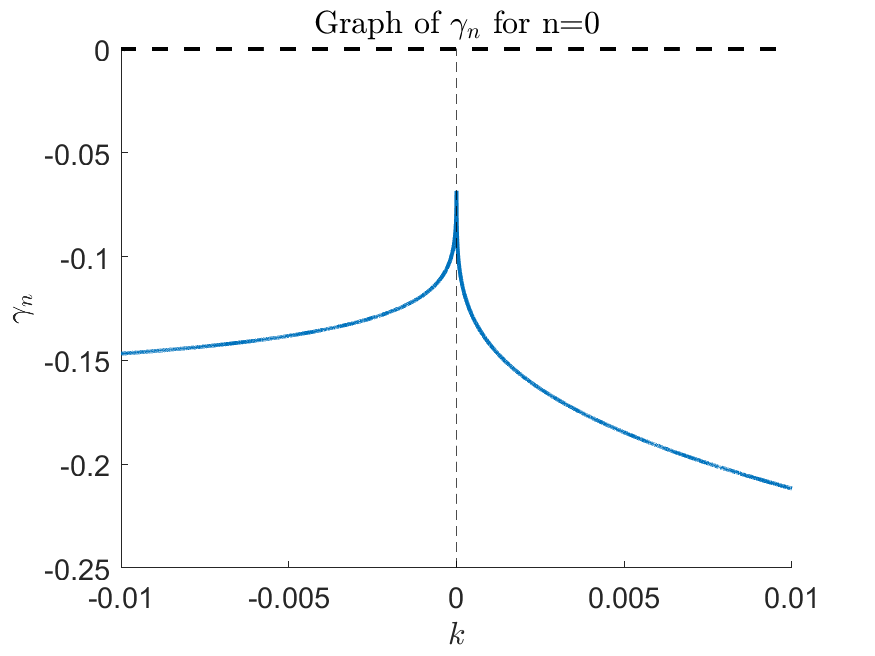
\includegraphics[width = .5\textwidth]{../Numerics/gamma_n0}
		\caption{Numerics for $n = 0$.}
	\end{figure}
	\begin{figure}
		\centering
		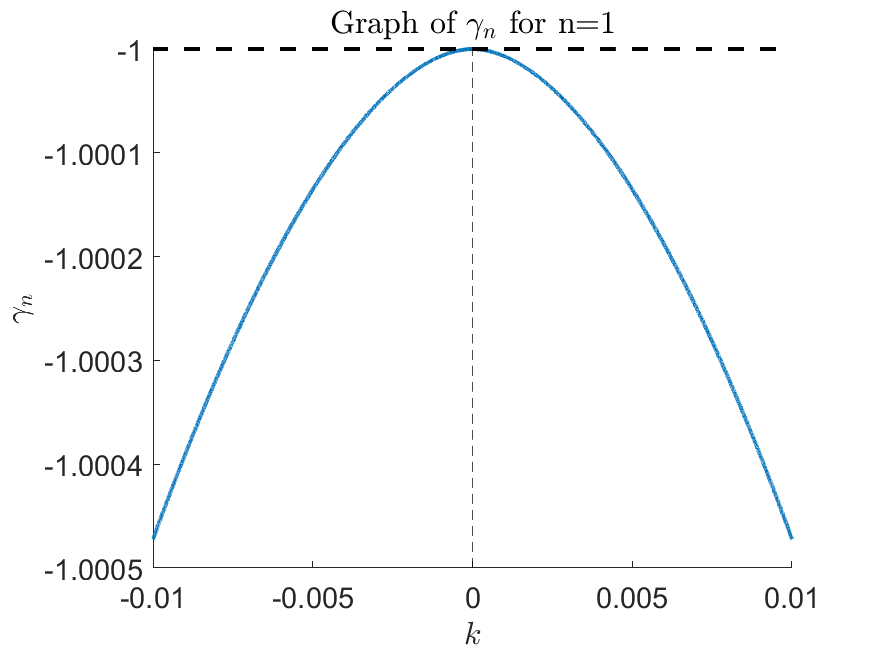
\includegraphics[width = .5\textwidth]{../Numerics/gamma_n1}
		\caption{Numerics for $n = 1$.}
	\end{figure}
		\begin{figure}
		\centering
		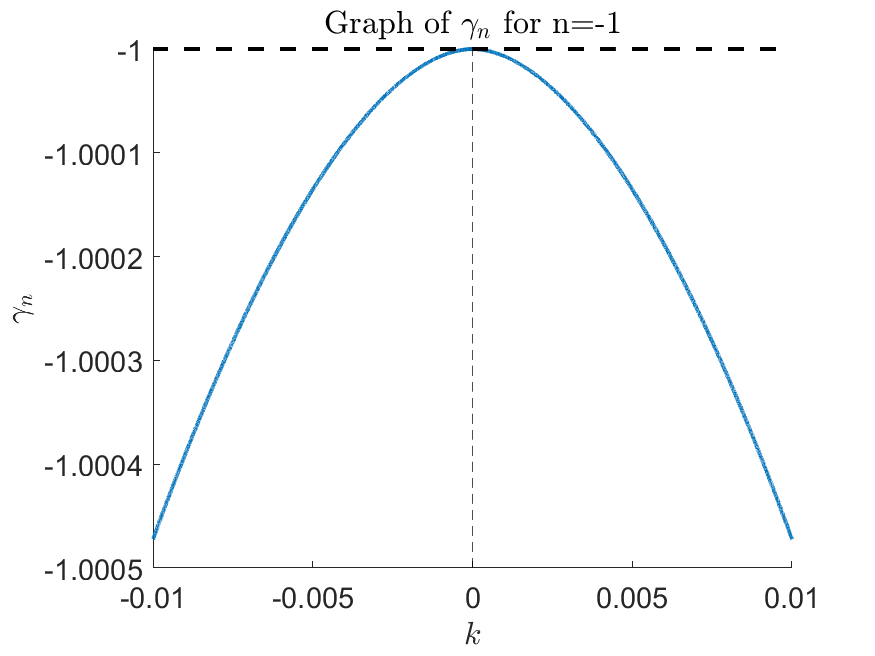
\includegraphics[width = .5\textwidth]{../Numerics/gamma_n-1}
		\caption{Numerics for $n = -1$.}
	\end{figure}
	\begin{figure}
		\centering
		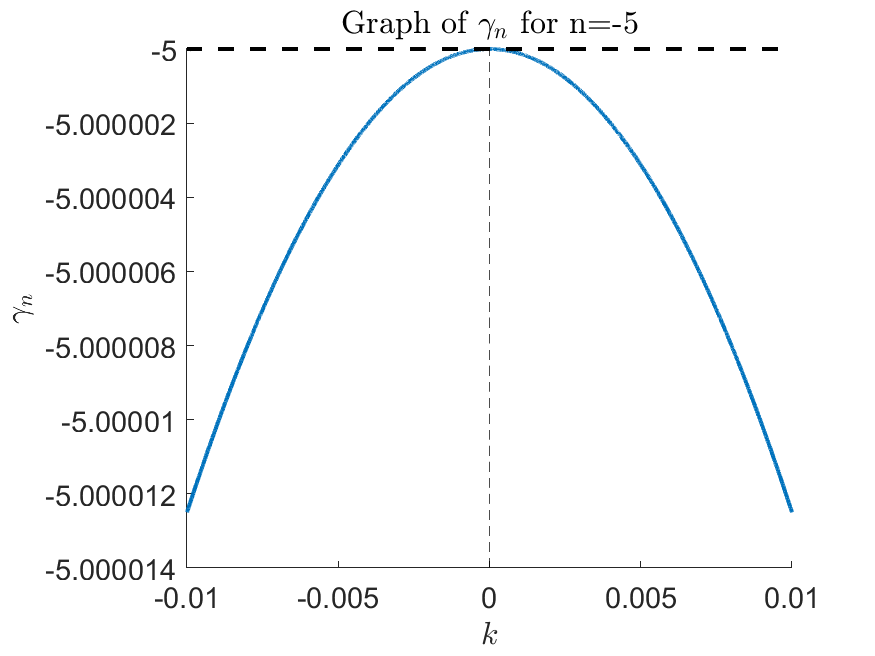
\includegraphics[width = .5\textwidth]{../Numerics/gamma_n-5}
		\caption{Numerics for $n = -5$.}
	\end{figure}
	\begin{figure}
		\centering
		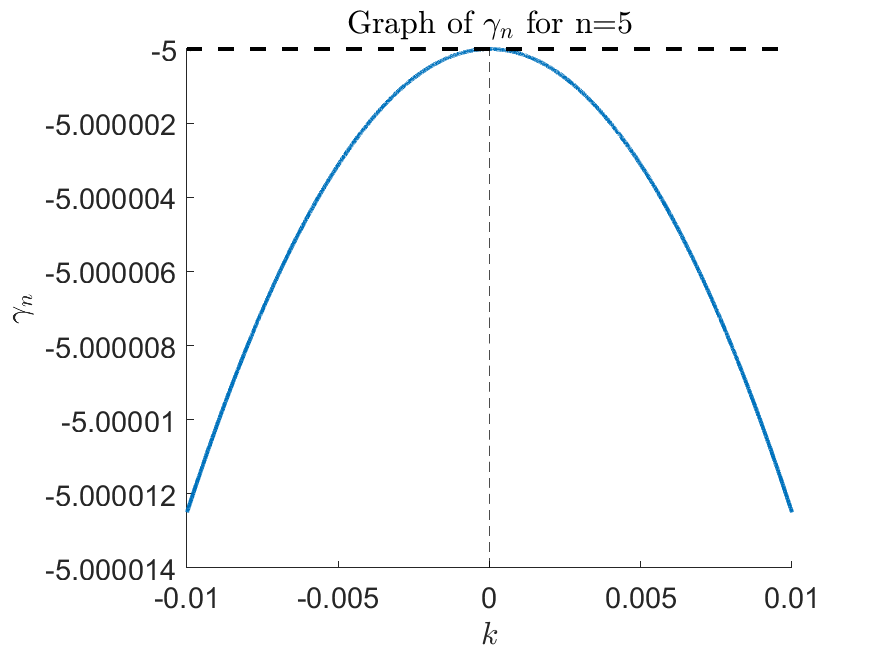
\includegraphics[width = .5\textwidth]{../Numerics/gamma_n5}
		\caption{Numerics for $n = 5$.}
	\end{figure}
	
\end{document}
